%%%%%%%%%%%%%%%%%%%%%%%%%%%%%%%%%%%%%%%%%%%%%%%%%%%%%%%%%%%%%%%%%%%%%%%%
% Escuela Politécnica Superior de la Universidad de Alicante
% Realizado por: Jose Manuel Requena Plens
% Contacto: info@jmrplens.com / Telegram:@jmrplens
%%%%%%%%%%%%%%%%%%%%%%%%%%%%%%%%%%%%%%%%%%%%%%%%%%%%%%%%%%%%%%%%%%%%%%%%

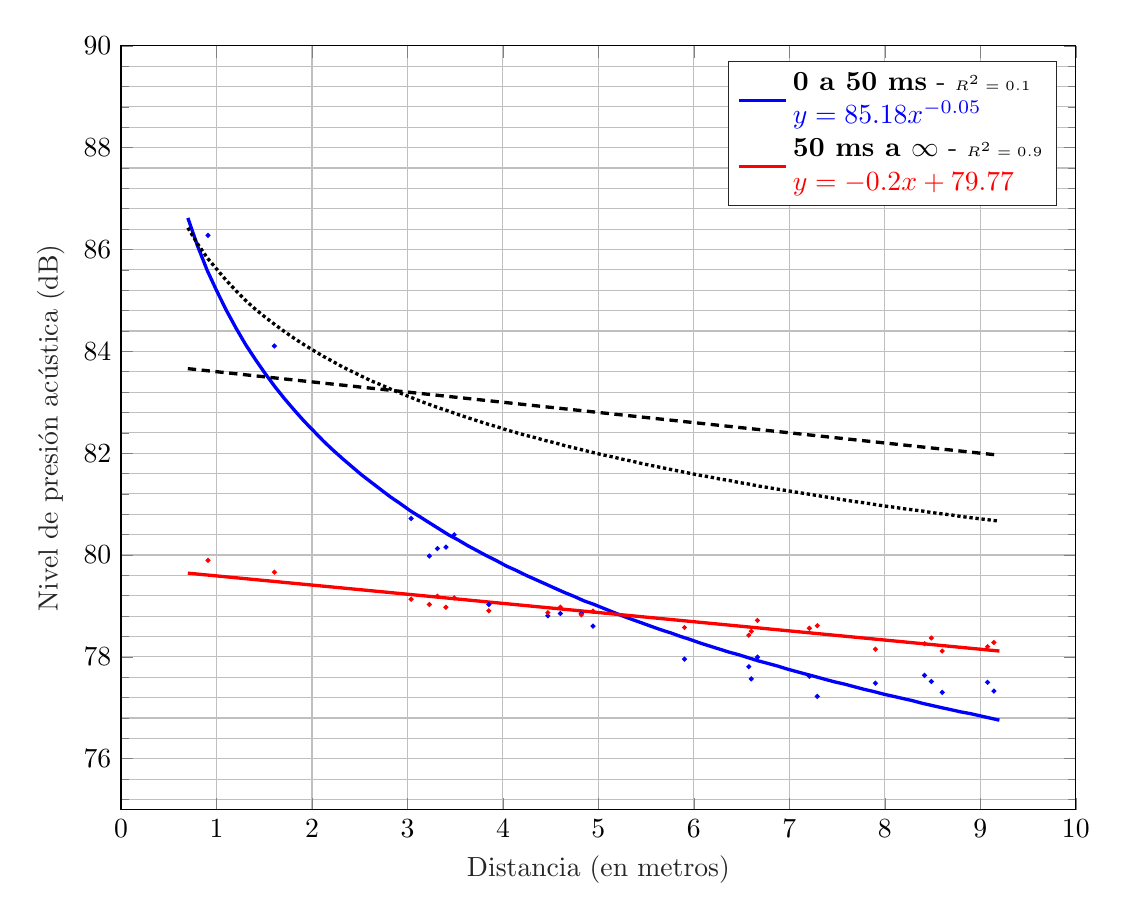
\begin{tikzpicture}

\begin{axis}[%
width=\textwidth,
height=0.8\textwidth,
at={(0\textwidth,0\textwidth)},
scale only axis,
xmin=0,
xmax=10,
xlabel style={font=\color{white!15!black}},
xlabel={Distancia (en metros)},
ymin=75,
ymax=90,
ylabel style={font=\color{white!15!black}},
ylabel={Nivel de presión acústica (dB)},
axis background/.style={fill=white},
xmajorgrids,
xminorgrids,
ymajorgrids,
yminorgrids,
minor y tick num= 4,
legend style={legend cell align=left, align=left, draw=white!15!black}
]
% Curvas EASE
\addplot[color=blue,domain=0.7:9.2, samples=85,line width=1.2]{85.18*x^(-0.047)};
\addlegendentry{\textbf{0 a 50 ms} - \tiny{$R^2 = 0.1$}\\$\color{blue}y = 85.18·x^{-0.05}$}

\addplot[color=red,domain=0.7:9.2, samples=85,line width=1.2]{-0.18*x+79.77};
\addlegendentry{\textbf{50 ms a $\infty$} - \tiny{$R^2 = 0.9$}\\$\color{red}y = -0.2·x+79.77$}

% Curvas in situ
\addplot[color=black,densely dotted,line width=1.2pt,domain=0.7:9.2, samples=85]{76.9*x^(-0.03)+8.7};
\addplot[color=black,densely dashed,line width=1.2pt,domain=0.7:9.2, samples=85]{-0.2*x+75.1+8.7};

% Puntos
\addplot [color=blue, only marks,mark size=0.7pt]
  table[row sep=crcr]{%
 0.911043357914430	86.2772796781886\\
1.60623784042090	84.1056446478500\\
3.03809150619266	80.7162943773909\\
3.22955105239103	79.9791235432895\\
3.31360830515618	80.1257164588809\\
3.40293990543471	80.1549543981309\\
3.48998567332303	80.3976116923752\\
3.85259652701915	79.0293836816767\\
4.46989932772540	78.8058727354038\\
4.60217339960154	78.8512802176443\\
4.82104760399646	78.8496625245368\\
4.94393567919325	78.6032259795649\\
5.90169467187180	77.9558802268358\\
6.57495247131110	77.8065806803430\\
6.60151497763960	77.5670065559296\\
6.66558324529819	77.9950758659912\\
7.20971566707037	77.6179645821617\\
7.29246186140181	77.2229572843838\\
7.90126572138920	77.4832543472834\\
8.41605608346332	77.6356061014582\\
8.48704895708750	77.5171417313596\\
8.60116271209887	77.3035533865362\\
9.07634287585038	77.4993226551940\\
9.14220979851152	77.3278313594281\\
  };
  
  \addplot [color=red, only marks,mark size=0.7pt]
  table[row sep=crcr]{%
0.911043357914430	79.8951008237853\\
1.60623784042090	79.6634802579777\\
3.03809150619266	79.1311060267053\\
3.22955105239103	79.0290689238144\\
3.31360830515618	79.1915465704714\\
3.40293990543471	78.9738863429516\\
3.48998567332303	79.1574260253045\\
3.85259652701915	78.9034083062506\\
4.46989932772540	78.8673915409159\\
4.60217339960154	78.9747462523916\\
4.82104760399646	78.8249463712323\\
4.94393567919325	78.8986754815038\\
5.90169467187180	78.5761350266222\\
6.57495247131110	78.4254000607376\\
6.60151497763960	78.5015455533187\\
6.66558324529819	78.7147432854439\\
7.20971566707037	78.5621450983992\\
7.29246186140181	78.6112877631831\\
7.90126572138920	78.1512018038794\\
8.41605608346332	78.2574617650506\\
8.48704895708750	78.3698657405733\\
8.60116271209887	78.1141880570530\\
9.07634287585038	78.2003228792576\\
9.14220979851152	78.2818430326449\\
  };
\end{axis}
\end{tikzpicture}%